\subsection{Finding equilibria and bounds on parameters}

We recall that a \textit{steady state} of the system is a solution to the PDE, satisfying boundary conditions that does not depend on time, resulting in a vanishing time-derivative in equations. E.g., calling $\bm\psi$ a steady state of (\ref{eq:redu})-(\ref{eq:redw}), it holds
$$0 = \del_x^2 \bm\psi + \bm f(\bm\psi), \qquad \del_x \bm\psi(0) = \del_x\bm\psi(1) = 0.$$
By the look of things, an analytical derivation of all steady-states of this system seems a little bit too optimistic. That being said, one can look at \textit{constant steady-states} $\bar{\bm u} = (\bar u, \bar v, \bar w)$ with $\bar u, \bar v, \bar w \in \R$. Proceeding as such leads to the term $\del_x^2 \bar{\bm u}$ vanishing, the problem reformulates into a less daunting one: finding a triplet of reals $\bar{\bm u}$ such that
$$\bm f(\bar{\bm u}) = 0.$$

Since we proved in the last section that solutions with positive initial values will stay positive for all time $t>0$, we are only interested in \textit{positive} equlibria of the system. Depending on the choice of parameters, one shows that there is either one (stable), two (stable-unstable) or three (stable-unstable-stable) such steady-states. In each scenario, the origin $(0, 0, 0)$ is a stable equilibrium point . For a specific range of parameters, another stable, positive equilibrium arises whose value turns out to be one of the roots of some third-order polynomial. To build geometrical intuition, the reader can see constant steady states as the intersection points of 3 hypersurfaces (see \ref{fig:nullclines}) algebraically described by the reaction term, i.e., 
$$\text{Steady states} = \left\{\bm x \in \R^3 : \bigcap_{\kappa = f, g, h} \bigl\{ \kappa(\bm x) = 0 \bigr\}\right\}.$$
\begin{figure}
	\begin{tabular}{cc}
		\label{fig:nullclines}
		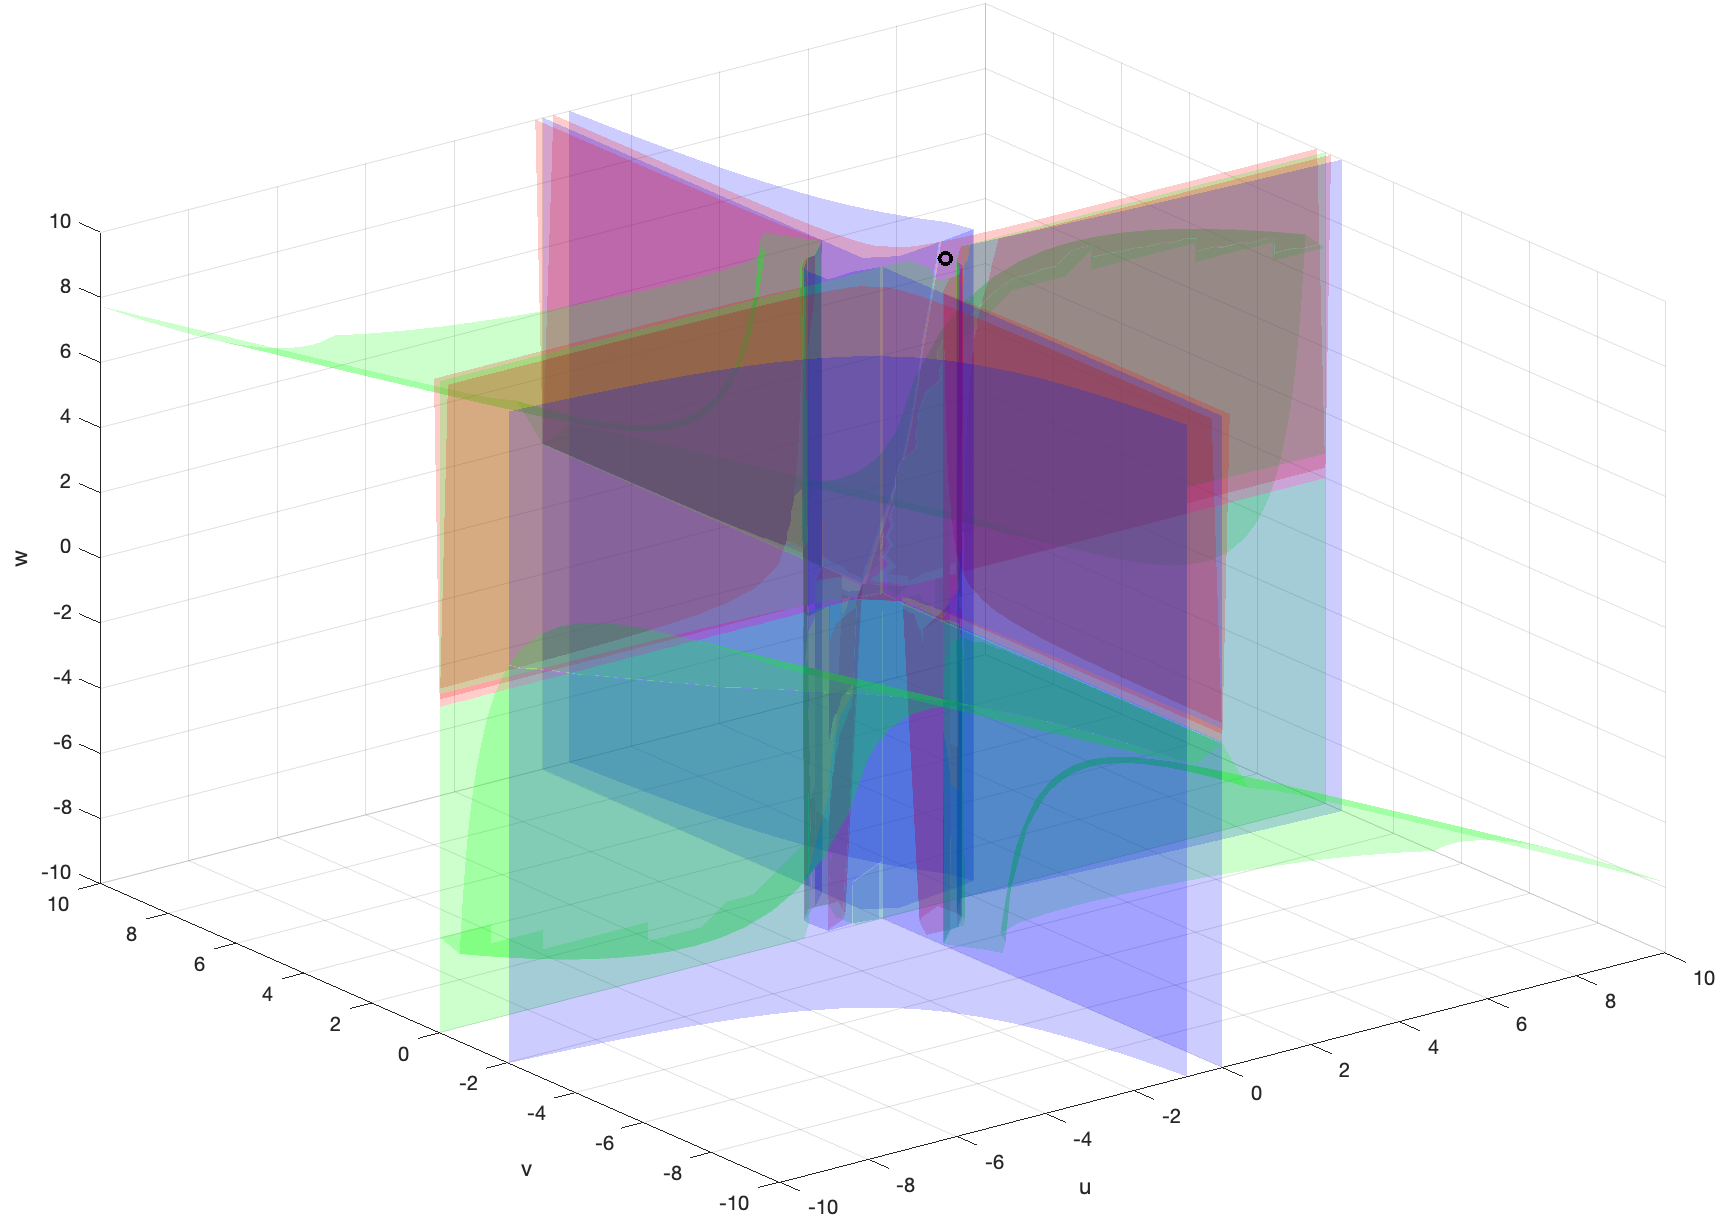
\includegraphics[width=0.49\linewidth]{figures/nullclines.png}
		&
		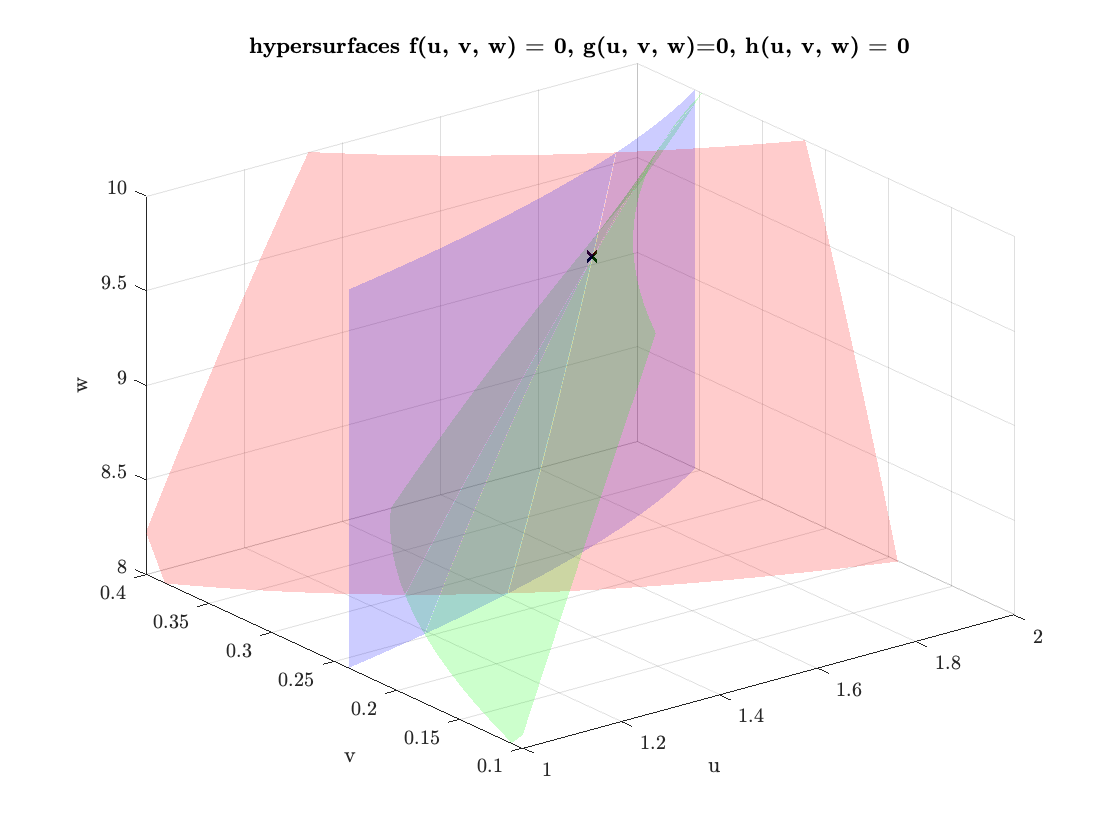
\includegraphics[width=0.49\linewidth]{figures/nullclines_zoom.png}
	\end{tabular}
\caption{Three-dimensional plot of the algebraic hypersurfaces associated to equations $f \equiv 0$ (blue), $g \equiv 0$ (green) and $h \equiv 0$ (red). The choice of parameters $\mu_f = 0.87, \mu_b = 0.68, \mu_l = 0.05, \mu_e = 0.60, m_1 = 5.36, m2 = 9.68, m3 = 17.27$ is made so that three steady-states exist. The figure on the left-hand panel is plotted over the domain $[-10, 10]^3$ while the right-hand panel plotted in a neighborhood of the non-zero stable steady-state.}
\end{figure}

\subsubsection{Analytical expression of constant steady-states}

The strategy here is to first find, if any, functions $\euH$ and $\euG$ such that $\bar u = \euH(\bar v)$ and $\bar w = \euG(\bar v)$ and then derive a condition on $\bar v$ to conclude. We formulate

%\begin{proposition}[Constant stationary solutions]
%	Let $\bar{\bm u} = (\bar u, \bar v, \bar w)$ be a constant steady-state of (\ref{eq:redu})-(\ref{eq:redw}). Then, either $ (\bar u, \bar v, \bar w) = (0, 0, 0)$ or $\bar u = \euH(\bar v), \bar w = \euG(\bar v)$
%	and all possible values of $\bar v$ are given by the roots of $\euP$ where
%	$$\euH(x) = \frac{m_1}{\mu_f + \mu_b x} - \frac{1}{x}, \qquad \euG(x) = \frac{m_3}{\mu_e}\left( 1 - \frac{\mu_f+ \mu_b }{m_1 x} \right), \qquad \euP(x) = ax^3 + bx^2 + cx + d$$
%	and the coefficients of $\euP$ are given by
%	\begin{align*}
%		a &= -\ml \mb - \frac{m_3 \mb}{\me} + \frac{m_3 \mb^2}{m_1 \me}, \\[0.5em]
%		b &= -\ml\mf + m_2\mb - \frac{m_2 \mb^2}{m_1} +\mb^2 - m_1\mb - \frac{m_3 \mf}{\me} + \frac{2 \mf\mb m_3}{\me m_1}, \\[0.5em]
%		c &= m_2\mf - \frac{2\mf\mb m_2}{m_1} + \mf\mb + \frac{m_3 \mf^2}{\me m_1}, \\[0.5em] 
%		d &= -\frac{m_2\mf^2}{m_1}.
%	\end{align*}
%\end{proposition}


\begin{proposition}[Constant stationary solutions]
	Let $\bar{\bm u} = (\bar u, \bar v, \bar w)$ be a constant steady-state of (\ref{eq:redu})-(\ref{eq:redw}). Then, either $ (\bar u, \bar v, \bar w) = (0, 0, 0)$ or $\bar u = \euH(\bar v), \bar w = \euG(\bar v)$
	and all possible values of $\bar v$ are given by the roots of $\euP$ where
	$$\euH(x) = \frac{m_1}{\mu_f + \mu_b x} - \frac{1}{x}, \qquad \euG(x) = \frac{m_3}{\mu_e}\left( 1 - \frac{\mu_f+ \mu_b }{m_1 x} \right)$$
	and  $\euP$ is given by
	
	\begin{multline}
		\euP{(x)} = \biggl(-\ml \mb - \frac{m_3 \mb}{\me} + \frac{m_3 \mb^2}{m_1 \me}\biggr)x^3 \\+ \biggl(-\ml\mf + m_2\mb - \frac{m_2 \mb^2}{m_1} +\mb^2 - m_1\mb - \frac{m_3 \mf}{\me} + \frac{2 \mf\mb m_3}{\me m_1}\biggr)x^2 \\ + \biggl(m_2\mf - \frac{2\mf\mb m_2}{m_1} + \mf\mb + \frac{m_3 \mf^2}{\me m_1}\biggr)x -\frac{m_2\mf^2}{m_1}.
	\end{multline}
\end{proposition}
\begin{proof}
	The proof consists of straightforward computations that are carried out in details in appendix [NOM APPENDIX].
\end{proof}

While this is quite a ludicrous task to achieve, one could derive the exact analytical expression for spatially homogeneous stationary solutions of (\ref{eq:redu})-(\ref{eq:redw}) using the cubic formula and by differentiating cases with positive (negative) discriminant to toss away imaginary roots. An important thing to notice is that some choices of parameters will lead $\euP$ to have roots $v$ such that one coordinate of $\bar{\bm u}$ is negative, or complex-valued. Since we always choose an initial condition $\bm u_0 > 0$, this is contradictory with the results proven in the last section. When this happens, it is an indicator that the system will converge towards the origin instead of another steady-state. \com{maybe try to find parameters such that only one root is positive and two are complex-conjugate, e.g. $(r_1, r_2, r_3) = (3, 1+i, 1-i)$ such that $\euH(r_1), \euG(r_1) > 0$ to see if it is possible to get another steady state that is not the origin.}

\begin{example}[Numerical computations of the roots]
	In MATLAB, we implement the polynomial $\euP$ as well as $\euG$ and $\euH$. We then use the function \texttt{roots} to find all eventual steady states (see figure (\ref{fig:matlabP})).
	\begin{figure}
		\label{fig:matlabP}
		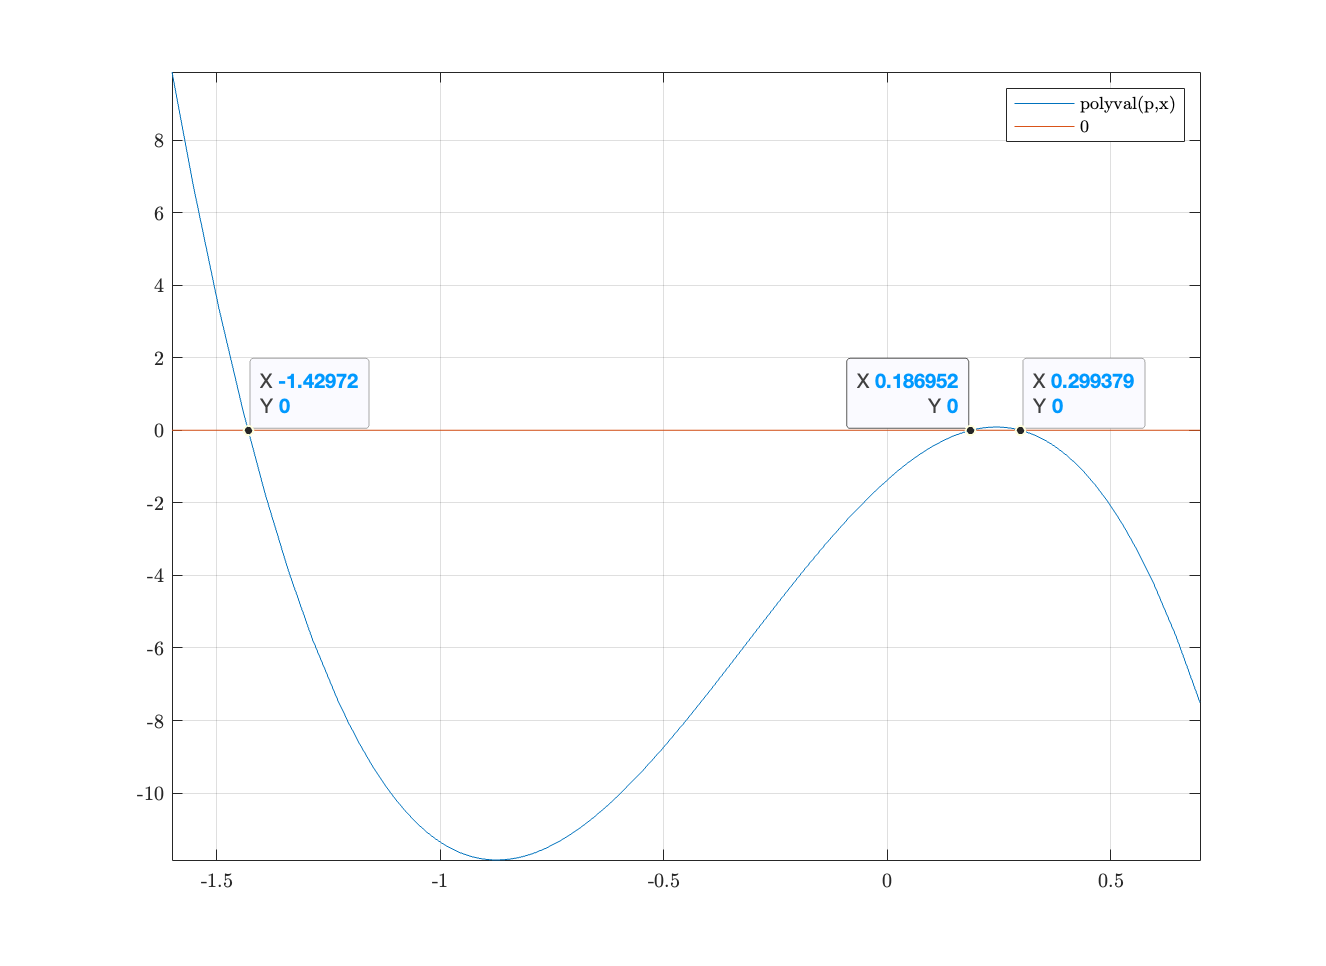
\includegraphics[width=0.6\linewidth]{figures/polyP_v.png}
		\caption{Roots of $\euP$ for $\mu_f = 0.87$, $\mu_b = 0.68$, $\mu_l = 0.05$, $\mu_e = 0.60$, $m_1 = 5.36$, $m2 = 9.68$, $m3 = 17.27$ (same parameters as in figure (\ref{fig:nullclines})) }
	\end{figure}
	Using the exact values returned by the machine, we find four steady-states 
	$$\bar{\bm u}_{3} = (0, 0, 0), \quad \bar{\bm u}_{2} = (-51.6587, -1.4300, 28.3989) $$
	$$\bar{\bm u}_{3} = (1.6527, 0.2994, 9.5284), \quad \bar{\bm u}_{4} = (0.0138, 0.1864, 0.0739)$$
	As previously mentioned, we can rule out $\bar{\bm u}_2$ because it has at least one negative coordinate. From there, using the Jacobian (computed in the next section) we can deduce the nature of $\bar{\bm u}_1, \bar{\bm u}_3, \bar{\bm u}_4$ and it reveals that the origin and $\bar{\bm u}_3$ are stable while $\bar{\bm u}_4$ is unstable.
\end{example}
	
	

\subsubsection{Snack break: finding bounds on asymptotically stable spatially homogeneous stationary solutions}

Assuming we know the values of the non-zero steady-state $\bar u, \bar v, \bar w$, one can use $f(\bar{\bm u}) = g(\bar{\bm u}) = h(\bar{\bm u})$ to derive a lower bound for each quantity. 

\begin{proposition}[Lower bounds on $\bm u$.]

Assume the parameters $m_1, m_2 > \mb$ and that $\bar u, \bar v, \bar w > 0$. Then 
	
\begin{center}
\begin{tabular}{c <{\hspace{2em}} c >{\hspace{2em}} c}
	$\bar u > \dfrac{\mf}{m_1 - \mb}$, & $\bar v > \dfrac{\ml}{m_2 - \mb}$, & $w >\dfrac{m_3}{\me}$
\end{tabular}
\end{center}
\end{proposition}

\begin{proof}
	We drop the $\bar{\cdot}$ (bar) notation for simplicity and start with $f(\bm u) = 0$. Substituting $f$ by its value from the system leads to
	$$0 = -\mf u + m_1 \frac{uv}{1 + uv} - \mb uv = u\biggl( -\mf + m_1 \frac{v}{1 + uv} - \mb v\biggr).$$
	We now use $\bar u \ne 0$ and rearrange the left-and-right-hand side.
	$$m_1 v = (\mf + \mb v) \underbrace{(1 + uv)}_{>1} > \mf + \mb v \quad\iff\quad v > \frac{\mf}{m_1 - \mb}$$
\end{proof}

\subsection{Linear dynamics and local behavior of the system}

In order to meet the required conditions for DDI, we first have to make sure system (\ref{eq:redu})-(\ref{eq:redw}) is stable in absence of diffusion when computed at a spatially homogeneous steady-state. This translates into saying that the Jacobian matrix $J = J_{\bm f}(u, v, w)$ of $\bm f$ at a steady-state satisfies $s(J) < 0$. A rapid computation shows

$$
J = \bpm  -\mu_f +  \dfrac{m_1v}{(1+u v)^2} - \mu_b v &  \dfrac{m_1 u}{(1+u v)^2} - \mu_b u & 0 \\[1.2em]
 \dfrac{m_2 v}{(1+u v)^2} - \mu_b v   & -\mu_l + \dfrac{m_2 u}{(1+u v)^2} - \mu_b u - w  & -v \\[1.2em] 
  \dfrac{m_3 v}{(1+u v)^2} &  \dfrac{m_3 v}{(1+u v)^2} & -\mu_e \epm.
$$

When working around the origin, it is perfectly fine to work with $J$ as it is. However, this form turns out to be rather impractical to work with when carrying out later computations around the other non-zero steady state. As a parry, we will later derive a set of useful equalities that will help us simplify the expression of $J$.

\subsubsection{In a neighborhood of the origin}

When taking $(u, v, w) = (0, 0, 0)$, almost all terms in the Jacobian disappear, leaving us with

$$
A(0, 0, 0) = \bpm  -\mu_f  &  0 & 0 \\[1.2em]
0  & -\mu_l & 0 \\[1.2em] 
0 & 0 & -\mu_e \epm
$$

which, by positivity of $\mu_f, \mu_b, \mu_e$ is unconditionally stable. Take a moment to convince yourself that in this case, there is no hope for DDI (to see why, notice that $\tr (A-\bm\mu D) < 0$ and $\det (A-\bm\mu D) = -\mu_f(\mu_l+ \bm\mu / \gamma)(\mu_e + \bm\mu d_2 / \gamma) < 0$ for all non-negative choices of $\bm\mu$). This tells us the system will always be stable, a statement that is corroborated by running a few simulations (see figure \ref{fig:simulations}).

\begin{figure}
	\centering
	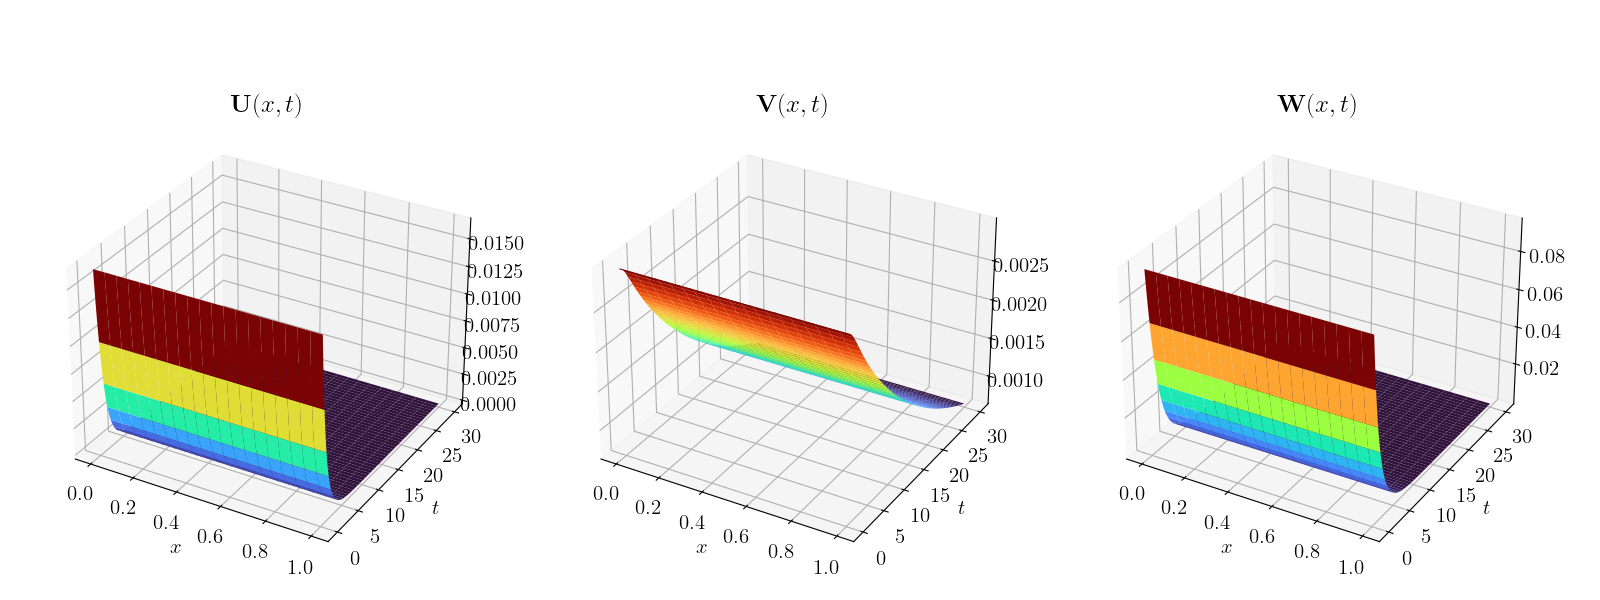
\includegraphics[width=\textwidth]{figures/stable_origin.png}
	\caption{space-time plot of numerical solutions $u, v, w$ to (\ref{eq:redu})-(\ref{eq:redw}) with constant initial condition $\bm X_0 = (\uu_0, \vv_0, \ww_0)$ close to the origin. One clearly sees how each quantity converges towards 0}
	\label{fig:simulations}
\end{figure}

\subsubsection{Around the other steady state}

For the entirety of this part, we assume the steady state to be non-trivial (which, otherwise, would compromise most computations we carry on). Let us move our interest to the other stable steady state provided the choice of parameters allows it. Using the fact that each term $u, v, w$ is positive, we can derive the following equalities from $f(u, v, w) = g(u, v, w) = h(u, v, w) = 0$

\begin{equation}
	\label{new_identities}
		m_1 \dfrac{v}{1 + u v} = \mu_f +  \mu_b v \quad \quad
		m_2 \dfrac{u}{1 + u v}  = \mu_l +  \mu_b u + w \quad \quad
		m_3 \dfrac{ u v}{1 + uv} = \mu_e w
\end{equation}


\begin{theorem}[Routh-Hurwitz criterion of order 3]
	Take a matrix $M \in \euM_3(\R)$. Then all the roots of $\chi_M$ lie in the negative half-plane (i.e. $\sigma(M) \subset \R_{<0}$) if and only if
	$\Delta_i(M) > 0$ for $i=1, 2, 3$ holds, where we define
	\begin{align*}
		\Delta_1(M) &= -\tr(M) \\[0.7em]
		\Delta_2(M) &= -\tr(M) \sum_{i < j} \det(M_{ij}) + \det(M) \\[0.7em]
		\Delta_3(M) &= -\det(M) \Delta_2(M),
	\end{align*}
Alternatively, let $\Tilde{\chi}_{M}(\lambda) = a_0 + a_1 \lambda + a_2 \lambda^2 + \lambda^3$ be the normalized characteristic polynomial of $M$. Then all roots of $\Tilde{\chi}_M$ lie in the negative half-plane if and only if all coefficients are positive and $a_2 a_1 > a_0$.
\end{theorem}


\begin{definition}[Submatrices defined by a pair of indices]
	Consider a matrix $A \in \euM_n(\R)$, for any couple of distinct indices $(i, j)$ with $1 \le i, j \le n$, we introduce the notation $A_{ij}$ to be the $2 \! \times \! 2$-matrix whose entries are formed by the entries of $A$ on line and column $i, j$.
\end{definition}


\begin{proposition}[Characteristic polynomial of a $3\times3$ matrix] Consider a matrix $A \in \euM_3(\R)$ whose entries are the $a_{ij}$ for $1 \le i, j \le 3$. Then 
	$$\chi_A(\lambda) = -\lambda^3 + \tr(A) \lambda^2 - \lp \sum_{i < j} \det(A_{ij})\rp \lambda + \det(A)$$.
\end{proposition}


\begin{lemma}[Necessary condition for DDI] Let $B := A - \lambda D$ denote the matrix of the linearized system. We claim that we can obtain DDI if and only if $\det(B_{12}) < 0$ and 
	
\end{lemma}


\begin{remark}[Minimum] The function $\mu \longmapsto |J - \mu D|$ reaches its minimum at the point:
	
\begin{equation}
	\resizebox{\hsize}{!}{%
		$\mu_{\mathbf{\mathrm{min}}} = \dfrac{\gamma}{2}\left( \dfrac{1}{(1+uv)^2}\left( m_2 u -  \dfrac{m_1m_2uv + \mu_b^2 uv(1+uv)^4 - \mu_b(m_1 + m_2) uv(1+uv)^2}{m_1 v - \mu_f (1 + uv)^2 - \mu_b v(1+uv)^2} \right)-\dfrac{\mu_e}{d_2} - \mu_l - \mu_b u - w\right) \notag$  
	}
\end{equation}
Please do not make me compute $\det(A - \mu_{\textrm{min}} D)$ ;-;. Also
\begin{equation}
	\resizebox{\hsize}{!}{%
		$\mu_{\mathbf{\mathrm{min}}} > 0 \quad \iff\quad \mu_f \biggl(m_2 - \mu_b u (1 + uv)^2\biggr) > \left( \dfrac{\mu_e}{d_2} + \mu_l + w \right) \biggl( m_1 v - \mu_f(1+uv)^2 - \mu_b v (1 + uv)^2\biggr) \notag$  
	}
\end{equation}
\end{remark}



$$\frac{|A_{12}| + |A_{13}|d_2}{2a_{11} d_2}$$


$$\bar u \bar v > \frac{\ml\mf}{(m_1 -\mb)(m_2 - \mb)} > 1 (1)$$

$$|J_{12}| = A - (1 - u^2 v^2)B > 0 \quad \text{if} (1)$$

